\chapter{Introduction to Neutrino Physics}
\label{c:theoryIntro}

This chapter is aimed at giving an introduction to the physics used in the thesis.

\section{Research Goals}
This research aims to construct a prototype Magnetized Iron Neutrino Detector (MIND) at the European Organization for Nuclear Research (CERN) and understand the performance of the detector to reconstruct charged particle tracks at a test beam at CERN and neutrino interactions at a neutrino beam at the JPARC facility in Japan.

\section{Theory}\label{section:Theory}
While measuring radioactive beta decay in the first two decades of the 20th century, physicists discovered what was then an anomaly. At the time it was thought that beta decay occurred as a two body process in which a neutron ($n$) decays to a proton ($p$) and electron ($e^-$). If this were the case, the energy of the proton and electron should be discrete and add up to the energy of neutron. However experiments showed that the electron could have a continuous spectrum of energy values, violating the energy conservation law, as seen in \FigRef{fig:betaeng}. In order to solve this anomaly, a third particle, the neutrino ($\nu$), was postulated by Wolfgang Pauli \cite{4Pauli:Online} and then incorporated into the beta decay by Enrico Fermi \cite{5Wilson}. The neutrino was postulated as a neutral particle with mass of less than 1\% of the proton mass and a spin of 1/2. For consistency, the particle used in the beta decay was changed to be noted as the antineutrino with the electron flavour, or just electron antineutrino $\bar{\nu_e}$. The addition of another particle changed the decay to $n \rightarrow p + e^- + \bar{\nu_e}$ and introduced the weak interaction model, as seen in \FigRef{fig:beta}. 

\begin{figure}[h!]
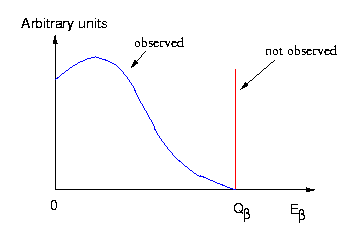
\includegraphics[width=\textwidth]{figures/NucleusBetaDecaySpectrum.png}
\caption{The kinetic energy spectrum of the emitted electron from beta decay (blue line). If no antineutrino were emitted the exact two body energy (red line) would be expected. \cite{31Nemo:Online}}
 \label{fig:betaeng}
\end{figure}

\begin{figure}[h!]
\centering
\begin{subfigure}{.5\textwidth}
  \centering
  \begin{fmffile}{badBeta}
\begin{fmfgraph*}(120,80)
\fmfstraight
\fmfleft{i1,i2,o1}
\fmfright{o2}

\fmf{fermion}{i1,v1}
\fmf{fermion}{v1,o1}

\fmf{boson}{v1,v2}
\fmf{fermion}{v2,o2}

\fmflabel{n}{i1}
\fmflabel{p}{o1}
\fmflabel{$e^{-}$}{o2}
\end{fmfgraph*}
\end{fmffile}
\vspace{2mm}
  \caption{The initial assumption beta decay}
  %\label{fig:sub1}
\end{subfigure}%
\begin{subfigure}{.5\textwidth}
  \centering
  \begin{fmffile}{beta}
\begin{fmfgraph*}(120,80)
\fmfstraight
\fmfleft{i1,i2,o1}
\fmfright{o2,o3}

\fmf{fermion}{i1,v1}
\fmf{fermion}{v1,o1}

\fmf{boson}{v1,v2}
\fmf{fermion}{v2,o2}
\fmf{fermion}{o3,v2}

\fmflabel{n}{i1}
\fmflabel{p}{o1}
\fmflabel{$e^{-}$}{o2}
\fmflabel{$\bar{\nu}_e$}{o3}
\end{fmfgraph*}
\end{fmffile}
\vspace{2mm}
  \caption{Correct beta decay}
  %\label{fig:sub2}
\end{subfigure}
\vspace{2mm}
\caption{Feynman diagrams showing beta decay.}
\label{fig:beta}
\end{figure}

It would take another twenty years until the neutrino was experimentally discovered by the Savannah river reactor experiment in 1956~\cite{6Reines} and awarded the Nobel prize in 1995.

After the discovery of the electron neutrino ($\nu_e$), several neutrino experiments were performed and led to the discovery of two other neutrino types/flavours, the muon neutrino ($\nu_\mu$) and the tau neutrino ($\nu_\tau$)~\cite{7Danby, 8Perl, Fix1}.

\subsection{Standard Model neutrino}\label{subsection:SMN}
The standard model of particle physics or simply the Standard Model (SM) categorizes all the fundamental particles that have been discovered experimentally and the mathematics of their properties and how they interact \cite{32Burchan:1995}. Currently there are two fundamental types of particles which are modelled as point like, quarks (fractional charge) and leptons (integer charge), seen in figure \FigRef{fig:standardModel}. Aside from these gauge bosons, the force mediators, are in the standard model. The split can also be seen as ferminos (fractional spin) and bosons (integer spin). \textbf{All gauge bosons are bosons (as the name implies) and all quarks and leptons are fermions.}

\begin{figure}[h!]
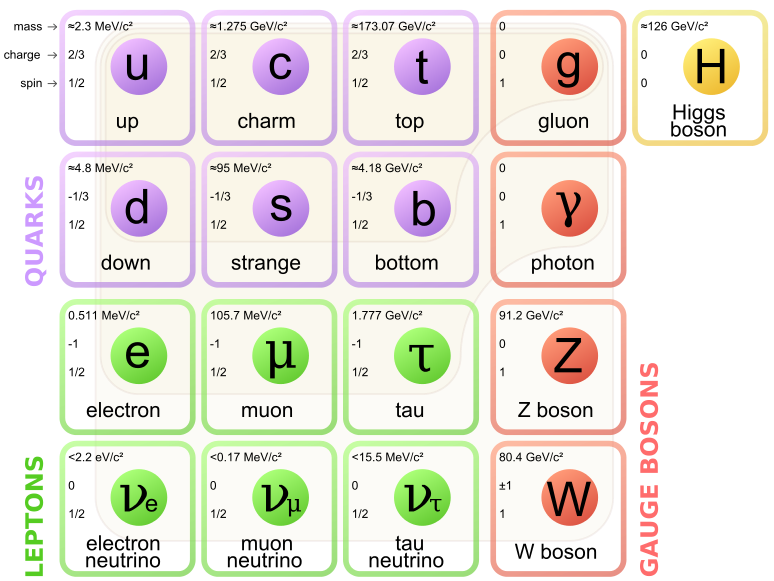
\includegraphics[width=\textwidth]{figures/Standard_Model_of_Elementary_Particles.png}
\caption{The standard model of particle physics where the three first columns represent the so called generations, starting with the first. \cite{33wiki1:Online}}
 \label{fig:standardModel}
\end{figure}

The experiment by \citeauthor{1Helicity} concluded that neutrinos only exist in a left handed chiral state, meaning that momentum and spin are oppositely aligned. They also concluded that anti-neutrinos only exists in the right handed state \cite{1Helicity}. In the initial or unexpanded SM, \cite{34doi:10.1142/9789812562203_0002}, only fermions which have both chiral states have mass through the Brout\hyp{}Englert\hyp{}Higgs mechanism~\cite{35Higgs}. At the time this lead to the definition of the neutrino as a massless particle, however in \SubSectionRef{subsection:Neutrinomassandoscillation} it will be shown that neutrino oscillations require at least one of the neutrinos to have mass. This indicates that the unexpanded SM needs to be extended to account for this new physics.

\subsection{Neutrino interactions}\label{subsection:Neutrino interactions}
As discussed previously, neutrino interactions are described by the weak interaction model. This model is split into two different parts depending on which boson mediates the interaction.
Charge Current (CC) interactions changes the final state quarks or leptons by one unit of electric charge and are mediated by the $W^+$ and $W^-$ bosons while Neutral Current (NC) interactions do not change the charge and are mediated by a $Z^0$ boson. 
To look at possible interactions of neutrinos described in the Standard Model of particle physics, one needs to look at the quantum field theory description of the interactions\cite{3Peskin, 2Hallsjo}. Sample Feynman diagrams showing these interactions can be seen in \FigRef{fig:CC} and \FigRef{fig:NC}.

\begin{figure}[h!]
\centering
\begin{subfigure}{.5\textwidth}
  \centering
  \begin{fmffile}{W+}
\begin{fmfgraph*}(120,80)
\fmfstraight
\fmfleft{i1,i2,o1}
\fmfright{o2,o3}

\fmf{fermion}{v1,i1}
\fmf{fermion}{o1,v1}

\fmf{boson,label=$W^{+}$}{v1,v2}
\fmf{fermion}{o2,v2}
\fmf{fermion}{v2,o3}

\fmflabel{$\bar{d}$}{i1}
\fmflabel{u}{o1}
\fmflabel{$e^{+}$}{o2}
\fmflabel{$\nu_e$}{o3}
\end{fmfgraph*}
\end{fmffile}
  %\caption{A subfigure}
  %\label{fig:sub1}
\end{subfigure}%
\begin{subfigure}{.5\textwidth}
  \centering
  \begin{fmffile}{W-}
\begin{fmfgraph*}(120,80)
\fmfstraight
\fmfleft{i1,i2,o1}
\fmfright{o2,o3}

\fmf{fermion}{i1,v1}
\fmf{fermion}{v1,o1}

\fmf{boson,label=$W^{-}$}{v1,v2}
\fmf{fermion}{v2,o2}
\fmf{fermion}{o3,v2}

\fmflabel{d}{i1}
\fmflabel{$\bar{u}$}{o1}
\fmflabel{$e^{-}$}{o2}
\fmflabel{$\bar{\nu}_e$}{o3}
\end{fmfgraph*}
\end{fmffile}
  %\caption{A subfigure}
  %\label{fig:sub2}
\end{subfigure}
\vspace{2mm}
\caption{Feynman diagrams showing an example of a charge current interaction.}
\label{fig:CC}
\end{figure}

\begin{figure}[h!]
\centering
  \begin{fmffile}{Z}
\begin{fmfgraph*}(120,80)
\fmfstraight
\fmfleft{i1,i2}
\fmfright{o1,o2}

\fmf{fermion}{i1,v1,o1}
%\fmf{fermion}{v1,o1}

\fmf{fermion}{i2,v2,o2}

\fmf{boson,label=$Z^{0}$}{v1,v2}
%\fmf{fermion}{o2,v2}
%\fmf{fermion}{v2,o3}

\fmflabel{$e^{-}$}{i1}
\fmflabel{$\nu_{\mu}$}{i2}
\fmflabel{$e^{-}$}{o1}
\fmflabel{$\nu_{\mu}$}{o2}
\end{fmfgraph*}
\end{fmffile}
  %\caption{A subfigure}
  %\label{fig:sub1}

\vspace{2mm}
\caption{Feynman diagram showing an example of a neutral current interaction.}
\label{fig:NC}
\end{figure}

From the Feynman diagrams one can calculate the probability of the interaction occurring, details can be found in \cite{3Peskin}. 

Looking at the following CC and NC examples \FigRef{fig:CMPNCCC} with electrons and muon neutrinos, so that the final states can be distinguished. The cross sections of both can be written as $\sigma_{CC} (\nu_\mu e^-) \approx \frac{G_F^2 s}{\pi} $ and $\sigma_{NC} (\nu_\mu e^-) \approx \frac{G_F^2 s}{\pi} \left[ (-\frac{1}{2} + \sin^2 \theta_W)^2 + \frac{1}{3}\sin^4 \theta_W\right] $ Giving a relation CC and NC as $\frac{\sigma_{CC}}{\sigma_{NC}} = 1/\left[ (-\frac{1}{2} + \sin^2 \theta_W)^2 + \frac{1}{3}\sin^4 \theta_W\right] \approx 11$. With the current values CC is approximately 11 times more likely to occur that NC.


\begin{figure}[h!]
\centering
\begin{subfigure}{.5\textwidth}
  \centering
  \begin{fmffile}{ECC}
\begin{fmfgraph*}(120,80)
\fmfstraight
\fmfleft{i1,i2}
\fmfright{o1,o2}

\fmf{fermion}{i1,v1,o1}
%\fmf{fermion}{v1,o1}

\fmf{fermion}{i2,v2,o2}

\fmf{boson,label=$W^-$}{v1,v2}
%\fmf{fermion}{o2,v2}
%\fmf{fermion}{v2,o3}

\fmflabel{$e^{-}$}{i1}
\fmflabel{$\nu_{\mu}$}{i2}
\fmflabel{$\nu_{e}$}{o1}
\fmflabel{$\mu^-$}{o2}
\end{fmfgraph*}
\end{fmffile}
  %\caption{A subfigure}
  %\label{fig:sub1}
\end{subfigure}%
\begin{subfigure}{.5\textwidth}
  \centering
  \begin{fmffile}{ENC}
\begin{fmfgraph*}(120,80)
\fmfstraight
\fmfleft{i1,i2}
\fmfright{o1,o2}

\fmf{fermion}{i1,v1,o1}
%\fmf{fermion}{v1,o1}

\fmf{fermion}{i2,v2,o2}

\fmf{boson,label=$Z^{0}$}{v1,v2}
%\fmf{fermion}{o2,v2}
%\fmf{fermion}{v2,o3}

\fmflabel{$e^{-}$}{i1}
\fmflabel{$\nu_{\mu}$}{i2}
\fmflabel{$e^-$}{o1}
\fmflabel{$\nu_{\mu}$}{o2}
\end{fmfgraph*}
\end{fmffile}
  %\caption{A subfigure}
  %\label{fig:sub2}
\end{subfigure}
\vspace{2mm}
\caption{Feynman diagrams with the same initial states.}
\label{fig:CMPNCCC}
\end{figure}

\subsection{Missing neutrinos}\label{subsection:Missing}

The Homestake experiment measured the flux of electron neutrinos and found only around 1/3 of the expected value from the theoretical model of the nuclear reactions in the core of the sun \cite{9Davis}. One of the possible explanations for the deficit was neutrino oscillations proposed by Bruno Pontecorvo~\cite{11Pontecorvo}. This theory was later verified at both the Sudbury Neutrino Observatory (SNO)~\cite{Fix6} and Super-Kamiokande~\cite{10Fukuda}. All three experiments were awarded Nobel prizes and have paved the way for physics beyond the Standard Model.

\subsection{Neutrino mass and oscillation in vacuum}\label{subsection:Neutrinomassandoscillation}
While looking at an analog of neutral kaon mixing for neutrinos Bruno Pontecorvo, in 1957, developed the concept of neutrino-antineutrino transitions~\cite{11Pontecorvo}. Even though to date no matter-antimatter oscillation had been observed, the concept formed the foundation of lepton mixing, which was developed by Maki, Nakagawa, and Sakata~\cite{12Maki} and refined into a neutrino flavour oscillation model by Bruno Pontecorvo. They managed to show that neutrino mixing is a natural outcome of adding neutrino mass to a gauge theory~\cite{11Pontecorvo}

The relation between the flavour and mass eigenstates can be expressed as,
\begin{equation}
\label{eq:eigenstates}
 \left| \nu_\alpha \right\rangle = \sum_{i} U^{*}_{\alpha i} \left| \nu_i \right\rangle,
 \left| \bar{\nu_\alpha} \right\rangle = \sum_{i} U_{\alpha i} \left| \bar{\nu_i} \right\rangle\
 \end{equation}
where
 $\left| \nu_\alpha \right\rangle $ is a neutrino with a fixed flavour, $\alpha$ is one of \{e,$\mu$,$\tau$\} and  $\left| \nu_i \right\rangle$ is a neutrino with a fixed mass.
$U$ is the Pontecorvo-Maki-Nagawa-Sakata (PMNS) matrix in \eqref{PMNS},
\begin{equation}
\label{PMNS}
\begin{aligned}
U ={} & 
 \begin{pmatrix}
 c_{12} & s_{12} & 0\\
  -s_{12} & c_{12} & 0\\
  0 & 0 & 1\\
 \end{pmatrix} 
  \begin{pmatrix}
 1 & 0 & 0\\
  0 & c_{23} & s_{23}\\
  0 & -s_{23} & c_{23}\\
 \end{pmatrix} 
   \begin{pmatrix}
 c_{13} & 0 & s_{13}e^{i\delta_{CP}}\\
  0 & 1 & 0\\
  -s_{13}e^{-i\delta_{CP}} & 0 & c_{13}\\
 \end{pmatrix} 
 \\
 & \times
  \begin{pmatrix}
1 & 0& 0\\
  0 & e^{i\phi_2} & 0\\
  0 & 0 & e^{i\phi_3}\\
 \end{pmatrix} 
 \end{aligned}
\end{equation}
where $s_{ij} = \sin\theta_{ij}$ and $c_{ij} = \cos\theta_{ij}$ with $\theta_{ij}$ the three mixing angles and $\delta_{CP}$, $\phi_2$ and $\phi_3$ are complex phases. The parameters $\phi_2$ and $\phi_3$ are only non-zero if neutrinos are their own antiparticles, which is still unknown at the time of writing this~\cite{13PDG}.

The interpretation is similar to that of a time-dependent quantum state, the probability of finding a neutrino in a specific state is related to the mass states through the PMNS matrix in which the elements are time dependent. It can also be thought of as a rotation in space. The derivations of the oscillation probability for assuming only two neutrinos and also for three neutrinos are often given in literature for instance it is given in \cite{34doi:10.1142/9789812562203_0002}. The three neutrino flavour state \ref{eq:eigenstates} in an initial beam evolves in time as:

\begin{equation}
\label{eq:eigenstatesTime}
 \left| \nu_\alpha (t) \right\rangle = \sum_{i} e^{-i E_i t} U_{\alpha i} \left| \nu_i \right\rangle\
 \end{equation}

Which gives the Probability of flavour evolution as 
\begin{equation}
\begin{aligned}
P_{\nu_\alpha \rightarrow \nu_\beta} (t) &= \left|  \langle \nu_\beta \left| \nu_\alpha     \right\rangle  \right|^2
& = \sum_{i,j} \left| U_{\alpha i} U_{\beta i}^* U{\alpha j}^* U_{\beta j} \right| \cos[(E_i - E_j)t -arg(U_{\alpha i} U_{\beta i}^* U{\alpha j}^* U_{\beta j} ) ]
\end{aligned}
\end{equation}

\begin{equation}
\label{eq:Energy-momentum}
E_\alpha = \sqrt{\vec{p}^2 + m_i^2} \approx \left| \vec{p} \right| + \frac{m_i^2}{2\left| \vec{p} \right|}
\end{equation}

Which can then be rewritten to depend on distance travelled by the beam (x) if using a relativistic approximation of the  energy-momentum relationship \ref{eq:Energy-momentum} as

\begin{equation}
\label{eq:Problength}
\begin{aligned}
P_{\nu_\alpha \rightarrow \nu_\beta} (x) &= \left|  \langle \nu_\beta \left| \nu_\alpha     \right\rangle  \right|^2
& = \sum_{i,j} \left| U_{\alpha i} U_{\beta i}^* U{\alpha j}^* U_{\beta j} \right| \cos[\frac{2\pi x}{L_{ij}} -arg(U_{\alpha i} U_{\beta i}^* U_{\alpha j}^* U_{\beta j} ) ]
\end{aligned}
\end{equation}
where the oscillation length $L_{ij} = \frac{4\pi  \left| \vec{p} \right| }{\left| m_i^2 - m_j^2 \right|}$ and $\vec{p}$ is the 3-momentum of our initial beam.

It can be seen that if $m_i^2 - m_j^2 = 0 $ this probability becomes $0$ which contradicts the experimental results. This means that atleast one of the neutrinos must have non-zero mass which currently is not explained through the Standard Model. Also that if $U_{\alpha i}$ is real, which is related to $\delta_{CP} = 0$, then $arg(U_{\alpha i} U_{\beta i}^* U_{\alpha j}^* U_{\beta j} ) = 0$.

Current experimental focus lies with trying to measure values for all of these parameters and one of the most interesting for understanding more about the Big Bang theory is the complex phase $\delta_{CP}$. This is known as the CP-violating phase which, if non-zero, would state that there is a difference between how normal and anti-neutrinos oscillate.

\subsection{CP-violation, baryogenesis and leptogenesis}
According to the current understanding of the Big Bang theory, matter and anti-matter were created in equal amounts\cite{14Berry}. This gives rise to one of the major unsolved problems in physics, where is all the anti-matter? If the answer was simply that antimatter exists somewhere else in the universe, then we should see the annihilation horizon, where matter and anti-matter interact, however there are no signs of this. There has also not been any sign of this in the cosmic background radiation\cite{14Berry}.

Through observations of the universe, much more matter has been found compared to anti-matter. One direct measurement was AMS-01, which measured the ratio of anti-helium to helium in the universe to be of the order of $10^{-6}$~\cite{15AMS1}. Another measurement, AMS-02 seems to confirm the first measurement and build on the results~\cite{16AMS2}. 
From these experimental results, a mechanism is needed to explain why the antibaryon component of the universe is $\sim 10^{-9}$ to that of baryons. As of now our current models can not account for the difference thus there must be unknown processes that account for this.

The unknown process has been split into two different fields, baryogenesis, looking at direct CP-violation in the baryon-antibaryon asymmetry and leptogenesis, CP-violation in the leptons that translates to a baryon asymmetry. Leptogenesis will be covered in this thesis as it relates to neutrinos also it should be added that there are theories which explain baryogenesis through leptogenesis.

If neutrinos violate CP (Charge, Parity) by their oscillations being different for neutrinos and anti-neutrinos, this could explain the matter anti-matter imbalance that has been observed. CP-violation exists in the Standard Model but it can not explain the observed difference~\cite{3Peskin}, and measurements of the CP-violation in neutrino oscillations have not yet been able to show any conclusive results~\cite{17Gonzalez}.

\subsection{Current theory of leptogenesis}
Basing on similar reasoning to the discussion above, andrei Sakharov proposed three necessary conditions that any interaction which would produce matter antimatter imbalance must satisfy~\cite{37Sakharov}. These conditions are:
\begin{itemize}
\item Baryon number violation.
\item C-and CP-violation.
\item Deviation from thermal equilibrium.
\end{itemize}

The first conditions is very important in that it related cosmological models with models in particle physics. It also gives us a way to produce an excess of baryons over anti-baryons, as long as there is no reverse interaction, hence requiring the C violation. CP-violation is needed to counteract the balancing as well and finally out of thermal equilibrium to get around CPT-symmetry. As briefly mentioned previously the second condition is fulfilled in the SM, but not enough, and the third can always be satisfied. \textbf{However there is no way of violating baryon number conservation in the SM.}

In \cite{36CRC} a number of viable scenarios for baryogenesis are briefly discussed for instance Grand Unified theories, heavy Majorana neutrinos and supersymmetry.

\subsection{How to detect neutrinos and neutrino oscillation}
There is currently no way of seeing neutrinos directly, in comparison to for instance photons. \textbf{For that matter, what is direct?} Thus all experiments are based on looking at indirect detection by detecting interaction products. For instance beta decay~\FigRef{fig:beta} or the inverse (the charge conjugate) beta decay. Similar processes exist for all flavours of neutrinos, and the general limit is that neutrinos only interact weakly. All of the interacting particles, sans the neutrino, deposit energy when passing through matter. This energy can be measured by constructing a detector out of scintillating material which converts this deposited energy to photons. Finally these photons can be detected through conventional photo-detectors.

By looking at the oscillation probability \eqref{eq:Problength} one can devise two main classes of experiments for neutrino oscillations.

Finding a distance x to the source where $P_{\nu_\alpha \rightarrow \nu_\alpha} (x) < 1$ it is possible to look at so called disappearance of the beam. At the detector, by comparing the expected neutrino flux to the observed one can provide evidence for neutrino oscillations. For the disappearing flavour there must be a probability, $P_{\nu_\alpha \rightarrow \nu_\beta} (x) > 0, \alpha=\beta$ for another flavour to appear. The second kind of experiment, denoted as appearance, is based on looking for interaction products which are impossible without oscillations. An example of this would be to see a positron from a muon neutrino beam. More on this can be found well described in~\cite{34doi:10.1142/9789812562203_0002} and examples of different detectors will be discussed in chapter~\ref{c:expIntro}.

\section{Current Theories to explain neutrino mass}
As discussed in subsection~\ref{subsection:SMN}, it is clear that without having both types of chiral, neutrinos can not have mass through Brout\hyp{}Englert\hyp{}Higgs mechanism~\cite{35Higgs}. What other methods could explain the reason for neutrino masses?

\subsection{Dirac neutrinos}
Did we miss some perhaps heavier neutrinos with the other chirality? Would have to add other neutrinos for with the chirality.

\subsection{Majorana neutrinos}
If they are neutral, thus anti and normal are the same particle. (Z boson mass) only chirality would distinguish them.

\section{Extended theories with neutrinos}
In this section some extended theories requiring more neutrinos or neutrinolike particles are presented.

\subsection{Neutrinoless double beta decay}

\subsection{Massive neutrinos as dark matter}
What is SUSY? What is a neutralio? Sterile neutrinos

What is dark matter? Why cold? Current ideas and theories? How does it relate to neutrinos? Or to neutralinos?

%==============================================================================
%\section{Thesis Statement}
%\label{c:intro:thesisstatement}

%This is a thesis statement. There are many like it, but this one is mine.


